\section{Além do usual}

Considere a seguinte configuração com potencial complexo e autovalores complexos ($\R^d = \R^2$)
\begin{equation}
	d = 2, \  n = 2, \  \V(z)=|z|^{2a} - \Re{(t z^a)},  \ W(x) = g(x) = \log{|x|},  \ \beta_N = \beta N^2,  \ \beta = 2.
	\label{Equation: Complex}
\end{equation}

\begin{figure}[ht]
	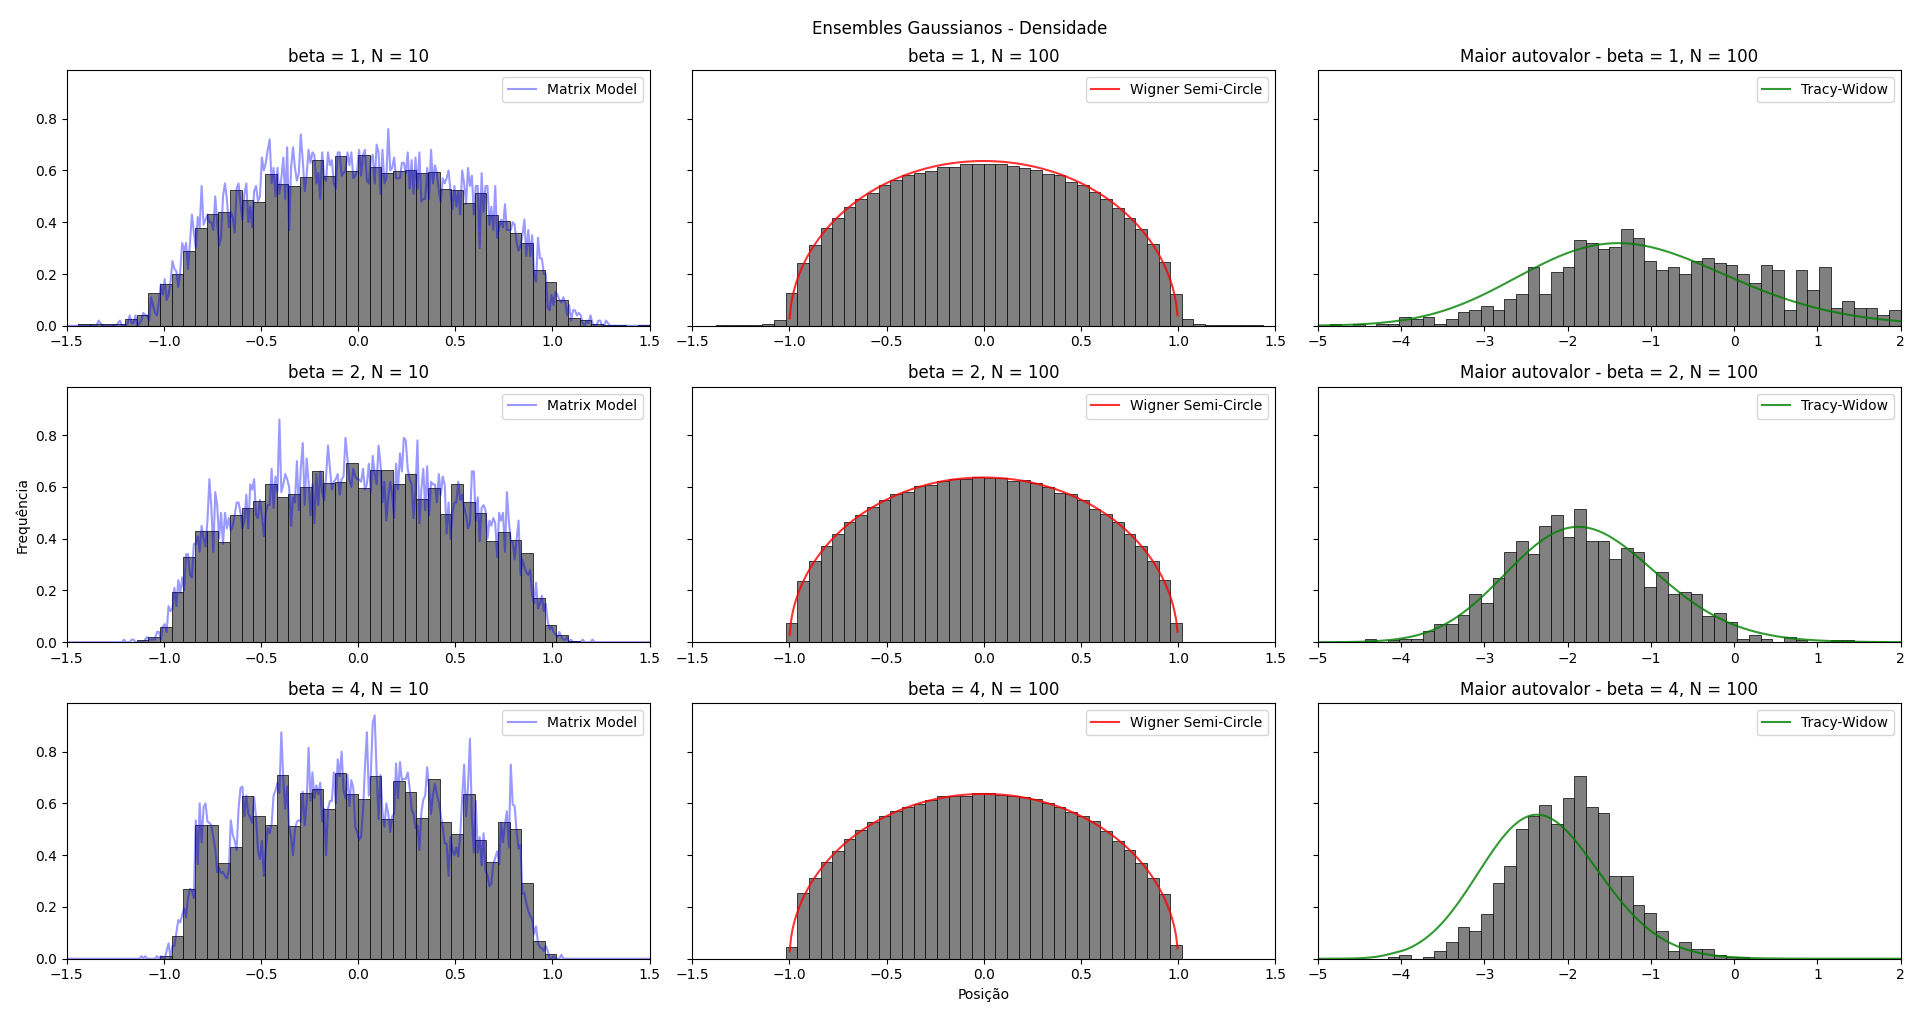
\includegraphics[width=\textwidth]{Assets/validationGaussianTracy.png}
	\caption{Medidas de equilíbrio para os ensembles gaussianos, equivalente à tomar \ref{Equation: Parametros Gaussian}. Para todos, vale a escolha de $\Delta t = 0.5$ e $nsteps = 2\cdot10^6$ passos, registrando a cada $1000$ iterações os microestados a partir da metade da simulação. Para as simulações à esquerda da figura se apresenta ainda a distribuição da amostragem de $10^6$ matrizes do tipo apropriado e a densidade resultante.}
	\label{Figura: Gaussian}
\end{figure}
